\documentclass{standalone}
%
\usepackage{tikz}
\usetikzlibrary{backgrounds,arrows.meta,shapes.callouts}
\usepackage{xcolor}
%
\definecolor{space}{HTML}{1F2C4E}
\definecolor{earth}{HTML}{0089FA}
\definecolor{craterm}{HTML}{616060}
\definecolor{linem}{HTML}{DBDBDB}
\definecolor{dida}{HTML}{FFDE00}
\definecolor{title}{HTML}{FBA706}
%
\usepackage{fontspec}
\setmainfont{Open Dyslexic}
%
\title{Vita di un asteroide}
\begin{document}
	\tikzset{
		notice/.style  = { draw, ellipse callout, callout relative pointer={#1} },
	}
	\begin{tikzpicture}[background rectangle/.style={fill=white},show background rectangle,>={[inset=0,angle'=27]Stealth}]
		%title
		\draw [black,ultra thick,fill=title] (0,9.8) rectangle (30,13.3);
		\node at (15,11.6) {\textcolor{black}{\fontsize{70}{71}\selectfont Il gioco dell'imitazione}};
		%
		\begin{scope}[shift={(0,1.5)}]
			\draw [ultra thick, fill=space] (1,0) rectangle (29,-2);
		\end{scope}
		%
		\begin{scope}[shift={(0,5)}]
			\draw [ultra thick, fill=earth] (20.5,4) rectangle (25.5,-4);
			\node at (23,0) {
\includegraphics[width=5cm]{img/personaggi/carl_sagan}};
			\node (example-textwidth-2) [notice={(3,0.5)}, ultra thick, right, align=center, text width=12cm, color=black, fill=white, font=\fontsize{23pt}{24pt}\selectfont] at (1,-1) {Il "gioco dell'imitazione" venne proposto da \textbf{Alan Turing} nel 1950 come possibile test per determinare se un computer era in grado di sviluppare un'intelligenza "umana".};
		\end{scope}
		% Protagonisti
		\begin{scope}[shift={(0,-21.5)}]
			\node at (4,14) {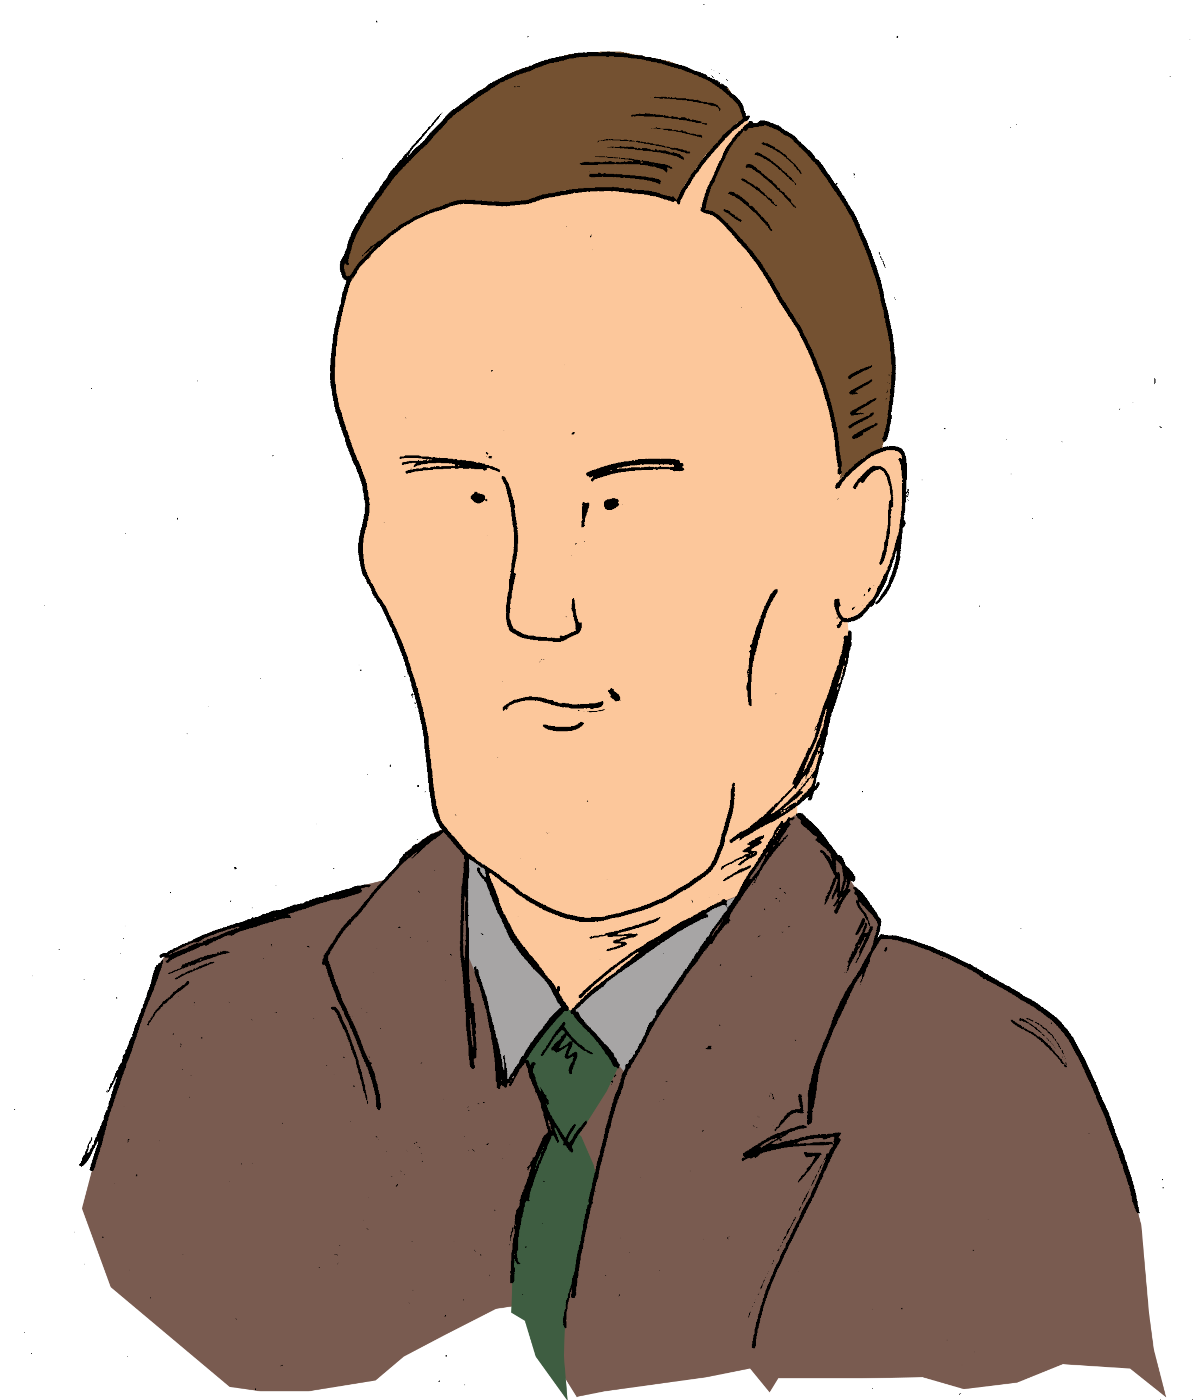
\includegraphics[width=8cm]{img/personaggi/alan_turing}};
			\draw [fill=earth!50!white, ultra thick] (1.3,8.2) rectangle (7,9.8);
			\node (example-textwidth-2) [right, align=left, text width=11cm, color=black, font=\fontsize{18pt}{19pt}\selectfont] at (1.5,9) {(C): Alan Turing};
			%
			\node at (15,14) {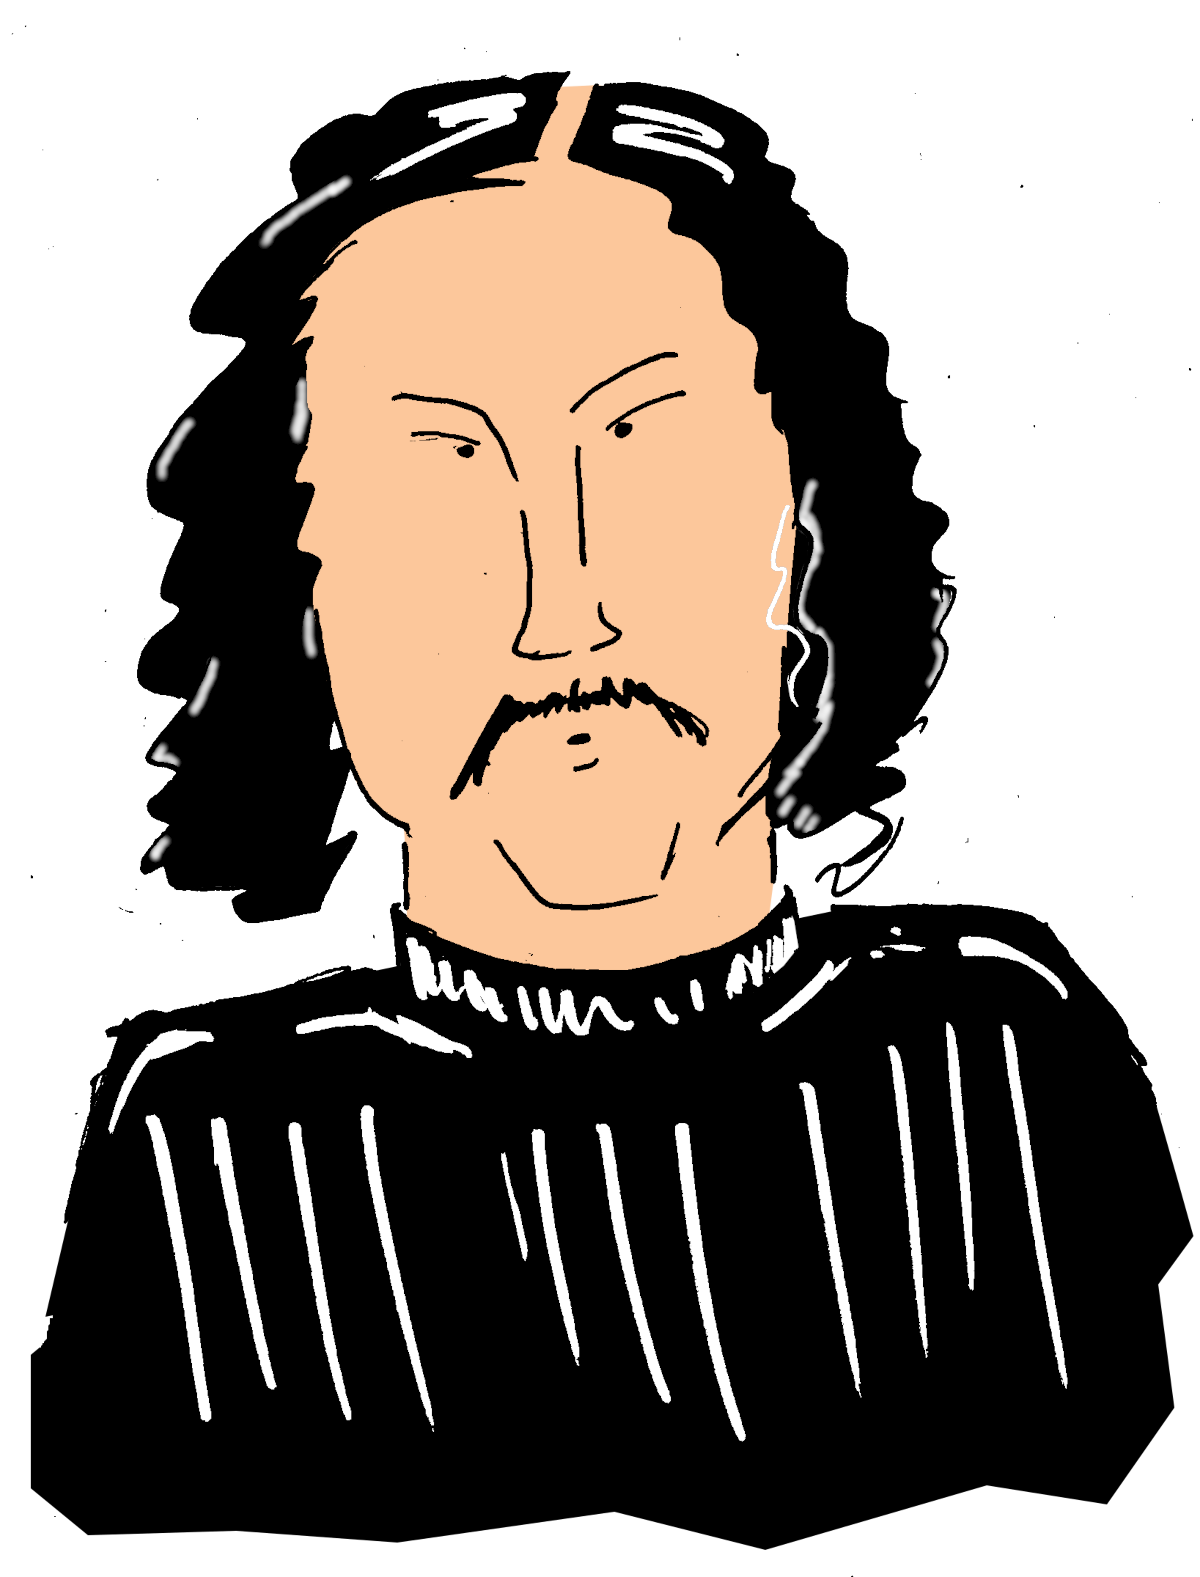
\includegraphics[width=8cm]{img/personaggi/christopher_strachey}};
			\draw [fill=earth!50!white, ultra thick] (10.3,8.2) rectangle (19.2,9.8);
			\node (example-textwidth-2) [right, align=left, text width=11cm, color=black, font=\fontsize{18pt}{19pt}\selectfont] at (10.5,9) {(A): Christopher Strachey};
			%
			\node at (25,14) {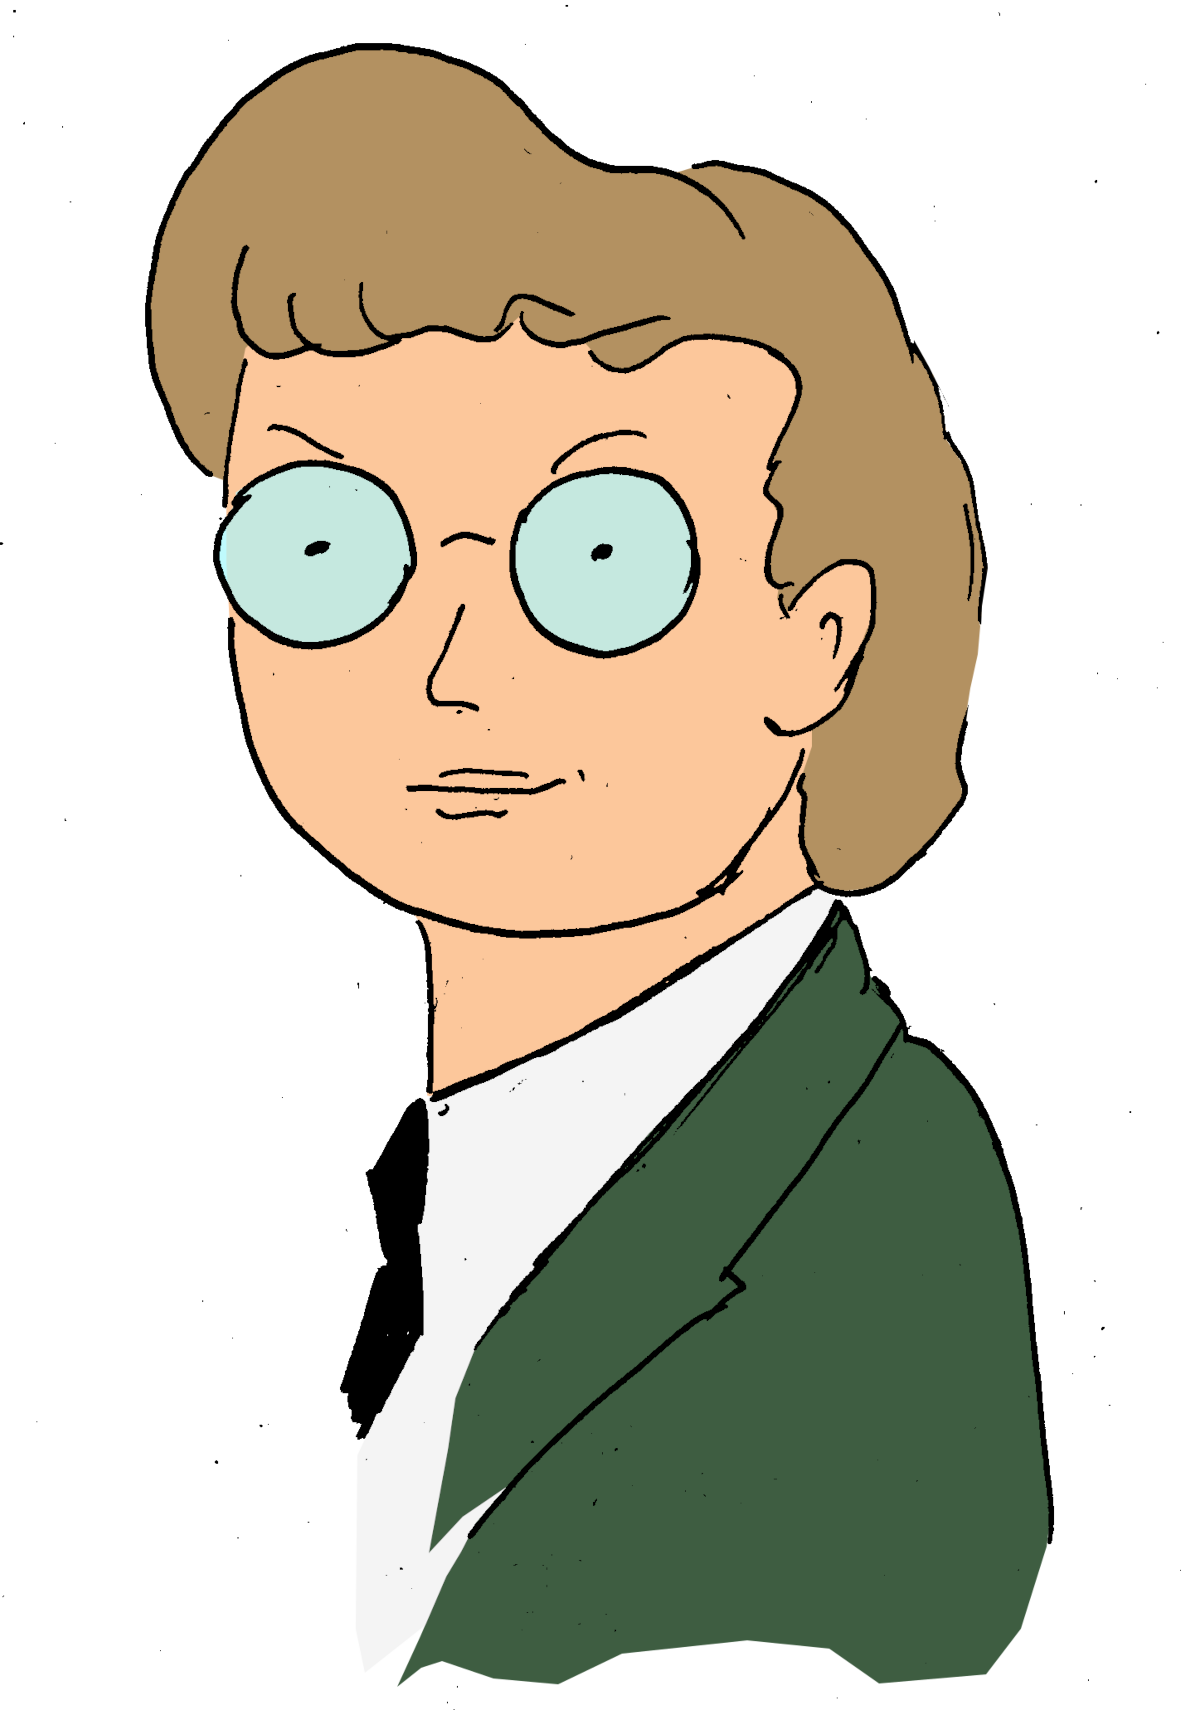
\includegraphics[width=8cm]{img/personaggi/joan_clarke}};
			\draw [fill=earth!50!white, ultra thick] (23.3,8.2) rectangle (29,9.8);
			\node (example-textwidth-2) [right, align=left, text width=6cm, color=black, font=\fontsize{18pt}{19pt}\selectfont] at (23.5,9) {(B): Joan Clarke};
			%
			\draw [fill=dida, ultra thick] (2,7) rectangle (27.5,4);
			%
			\node (example-textwidth-2) [right, align=left, text width=25cm, color=black, font=\fontsize{23pt}{24pt}\selectfont] at (2.5,5.5) {Il gioco viene giocato da tre persone, un operatore (C), un uomo (A) e una donna (B)};
		\end{scope}
		% Istruzioni
		\begin{scope}[shift={(0,-22)}]
			\node at (6,0) {
\includegraphics[width=5cm]{carl_sagan}};
			\node (example-textwidth-2) [notice={(-3,0.5)}, ultra thick, right, align=center, text width=12cm, color=black, fill=white, font=\fontsize{23pt}{24pt}\selectfont] at (10,-1) {L'operatore conosce le due persone solo con le etichette X e Y. Il suo obiettivo è quello di determinare chi dei due è uomo e chi donna.};
		\end{scope}
		% Gioco
		\begin{scope}[shift={(0,-32)}]
			\draw [fill=dida, ultra thick] (2,3.5) rectangle (27.5,1.5);
			\node (example-textwidth-2) [right, align=left, text width=25cm, color=black, font=\fontsize{23pt}{24pt}\selectfont] at (2.5,2.5) {L'operatore può porre varie domande a ciascuno dei due:};
			\node at (8,-4) {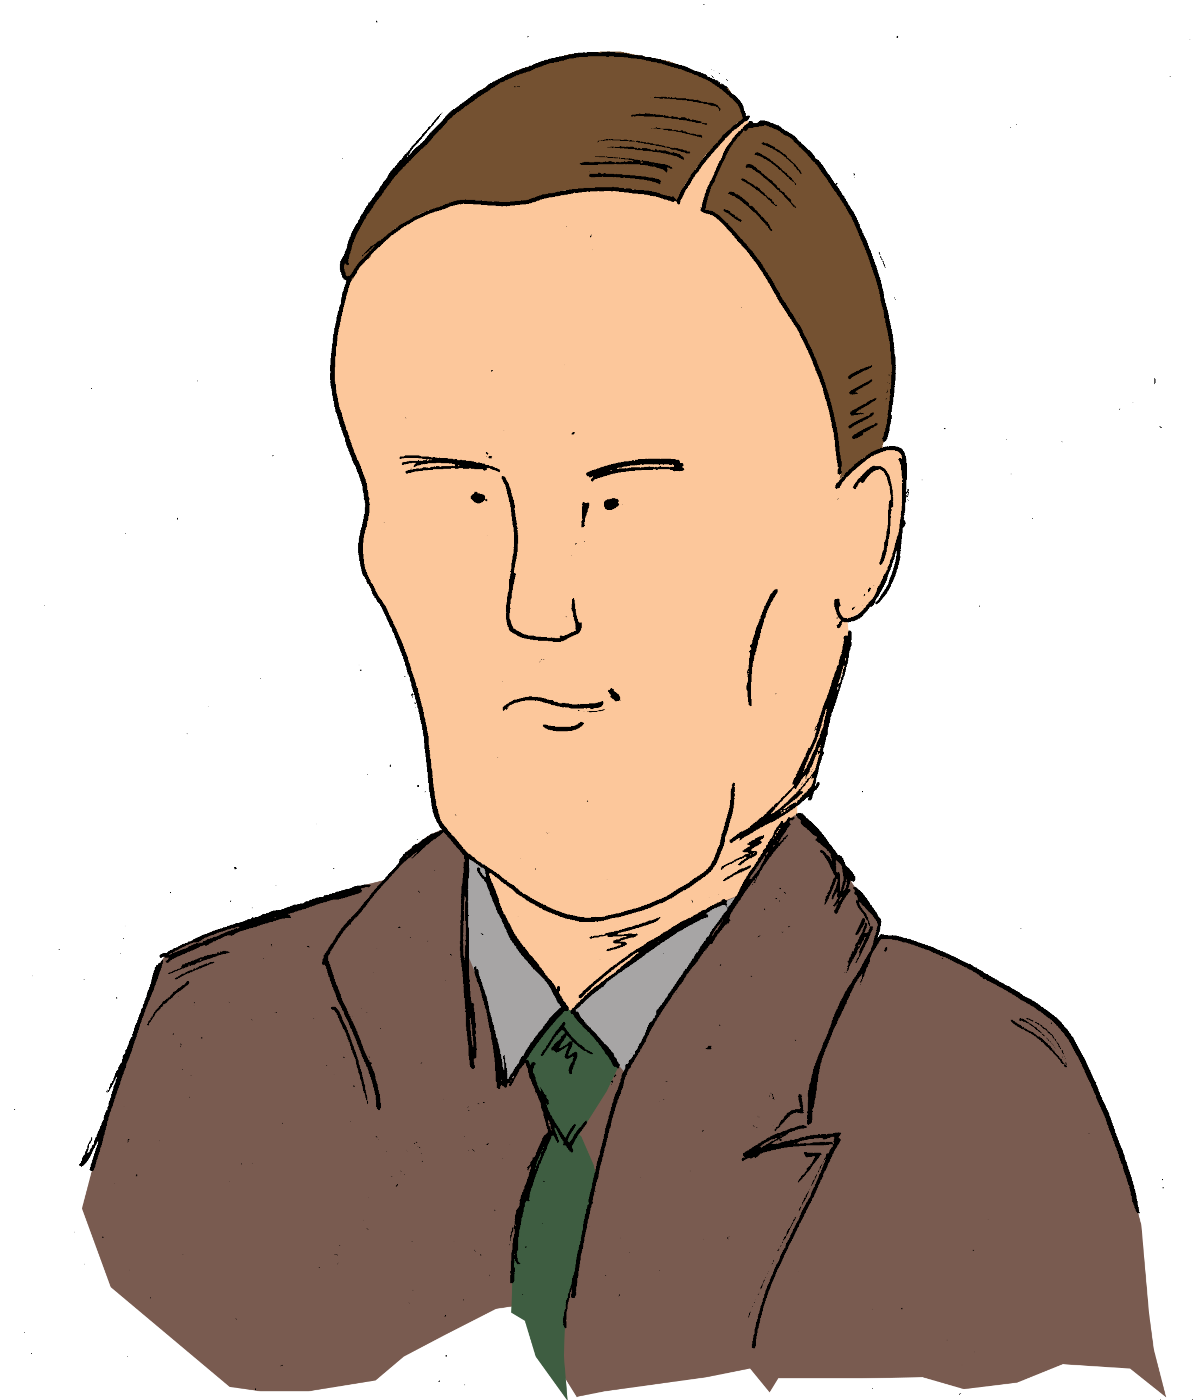
\includegraphics[width=8cm]{img/personaggi/alan_turing}};
			\node (example-textwidth-2) [notice={(-3,0.5)}, ultra thick, right, align=center, text width=12cm, color=black, fill=white, font=\fontsize{23pt}{24pt}\selectfont] at (12,-5) {Vuol dirmi X, per favore, la lunghezza dei propri capelli?};
			\node at (23,-12) {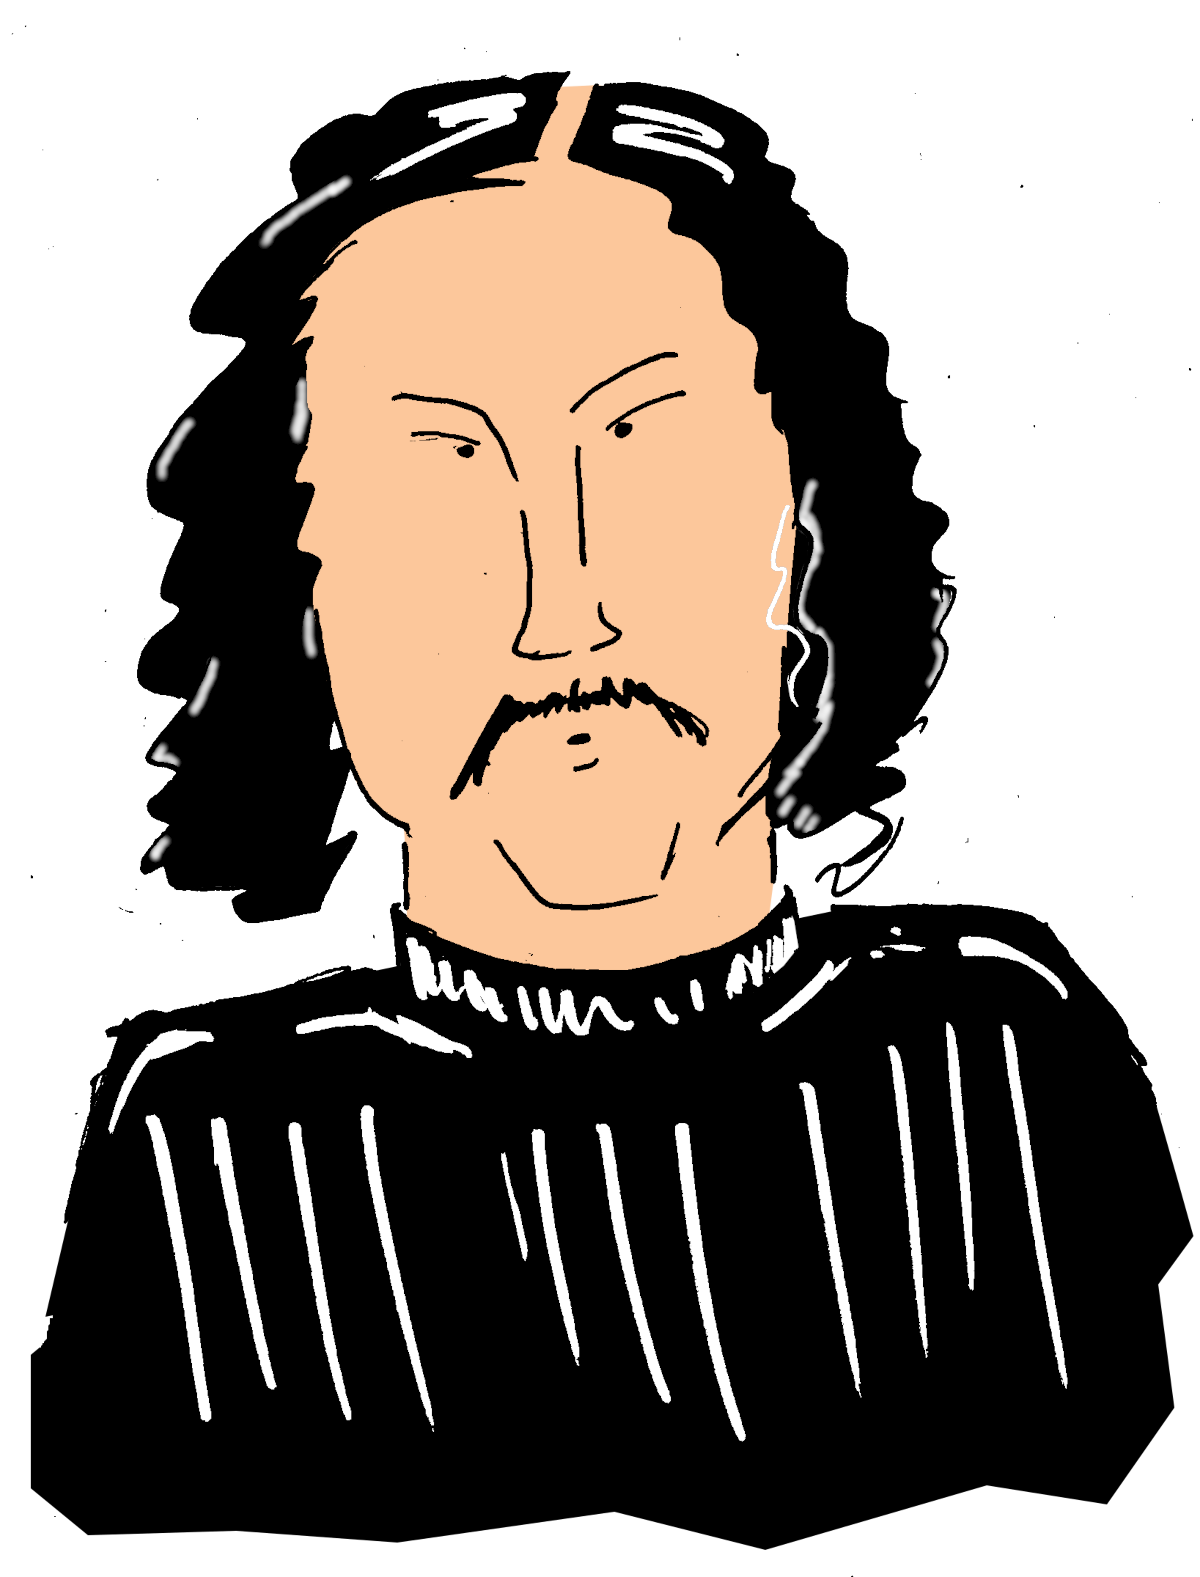
\includegraphics[width=8cm]{img/personaggi/christopher_strachey}};
			\node (example-textwidth-2) [notice={(3,0.5)}, ultra thick, right, align=center, text width=12cm, color=black, fill=white, font=\fontsize{23pt}{24pt}\selectfont] at (2,-13) {I miei capelli sono tagliati \emph{à la garçonne}, e i più lunghi sono di circa 25 centimetri};
			\node (example-textwidth-2) [right, align=left, text width=25cm, color=black, font=\fontsize{23pt}{24pt}\selectfont] at (2.5,2.5) {L'operatore può porre varie domande a ciascuno dei due:};
			\node at (8,-20) {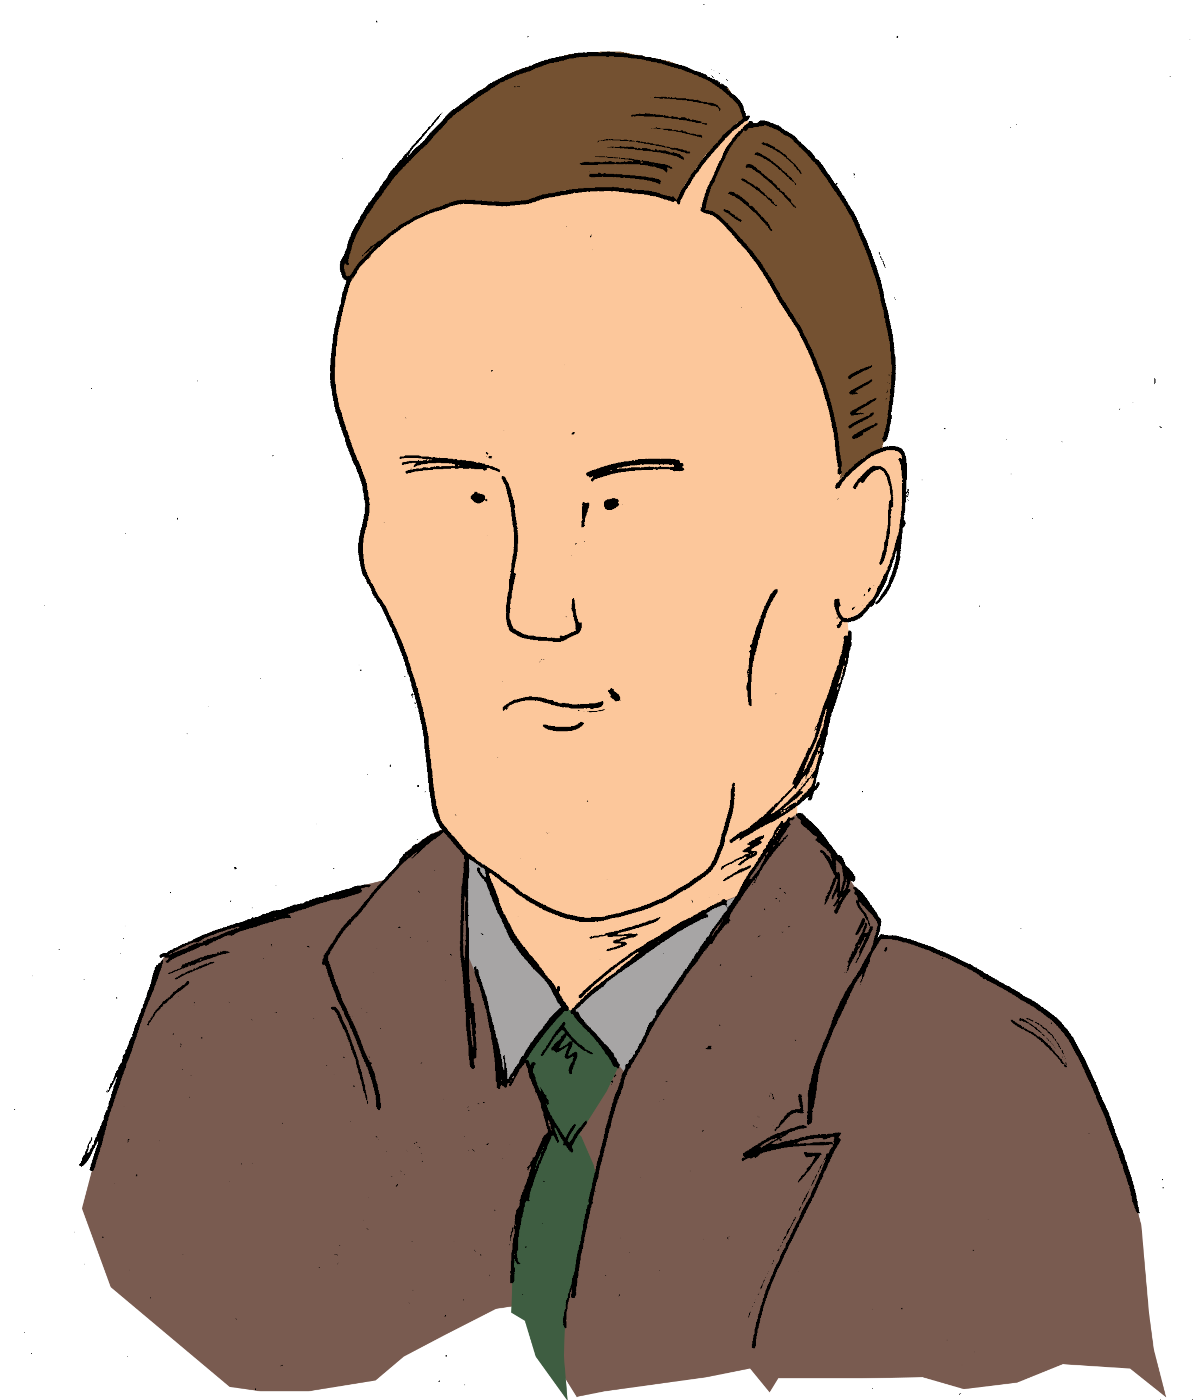
\includegraphics[width=8cm]{img/personaggi/alan_turing}};
			\node (example-textwidth-2) [notice={(-3,0.5)}, ultra thick, right, align=center, text width=12cm, color=black, fill=white, font=\fontsize{23pt}{24pt}\selectfont] at (12,-21) {Allora mi sa che è proprio X la donna!};
			\node at (23,-28) {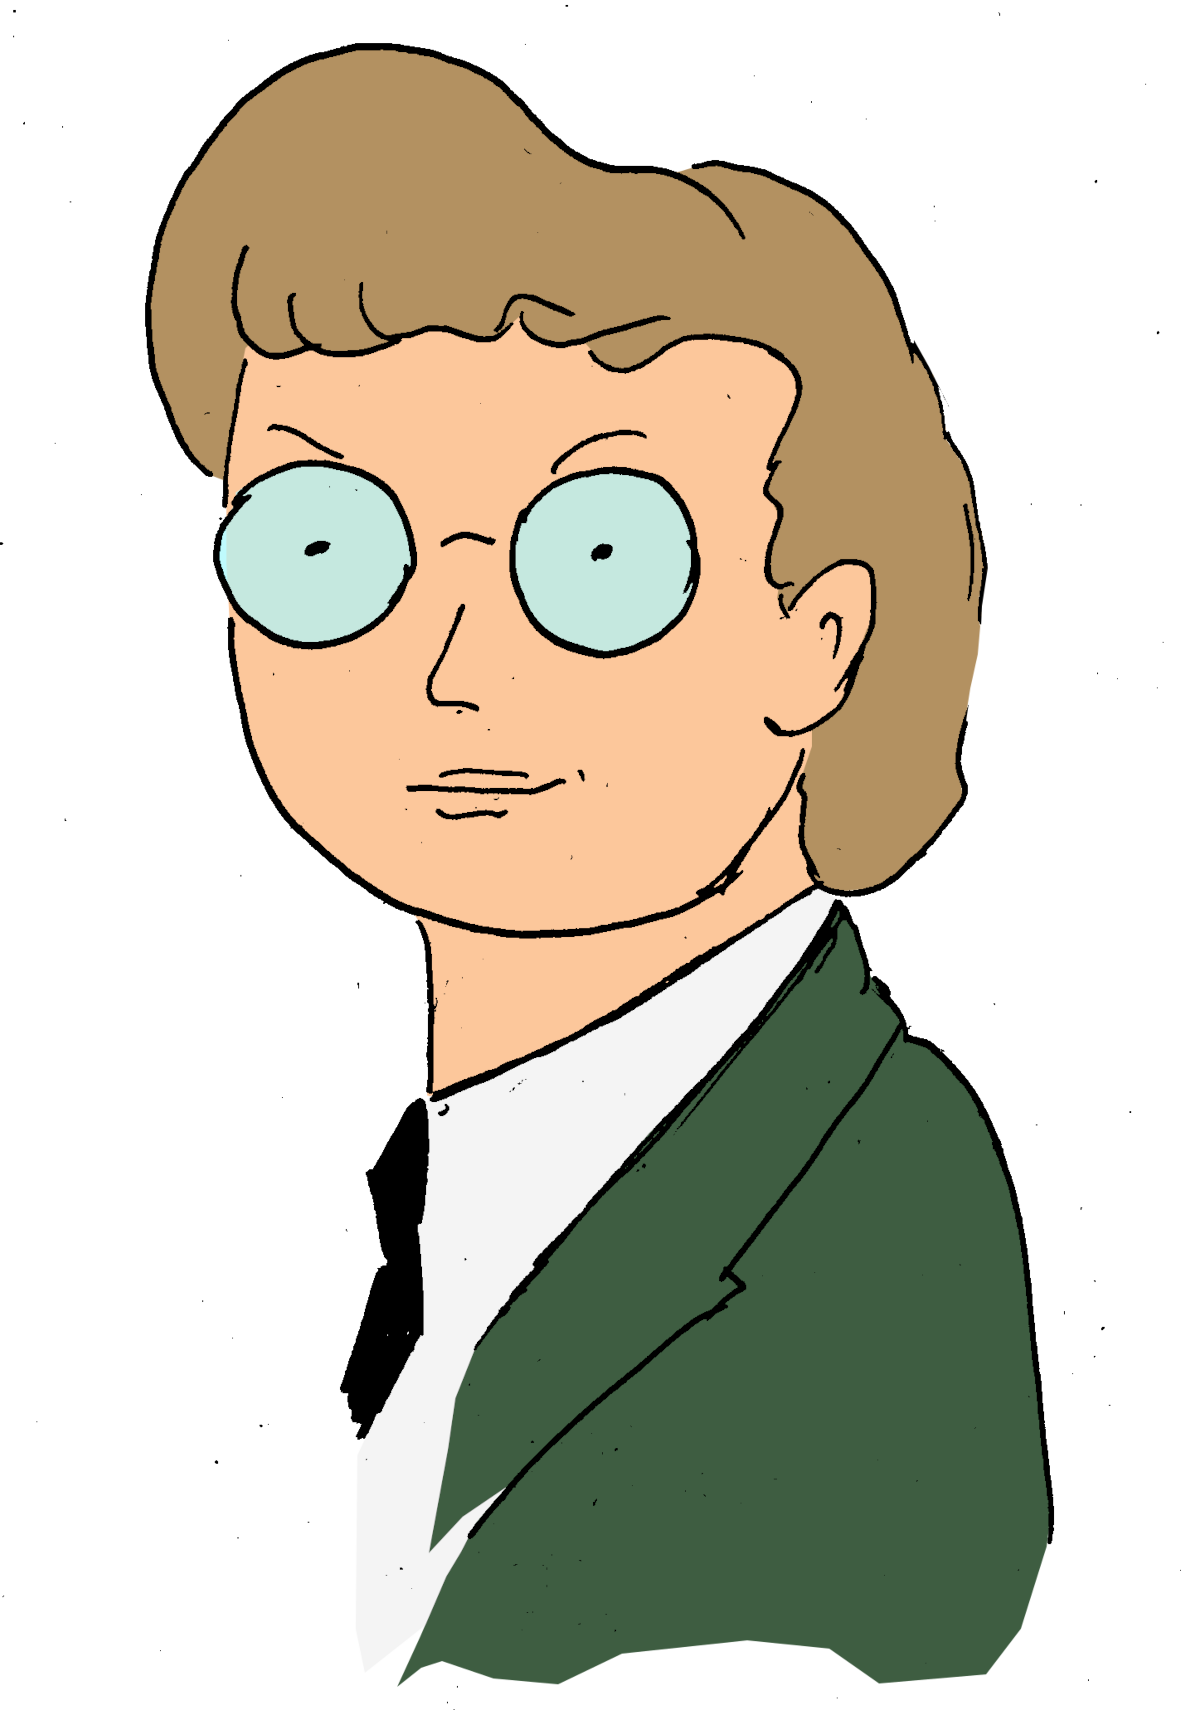
\includegraphics[width=8cm]{img/personaggi/joan_clarke}};
			\node (example-textwidth-2) [notice={(3,0.5)}, ultra thick, right, align=center, text width=12cm, color=black, fill=white, font=\fontsize{23pt}{24pt}\selectfont] at (2,-29) {Non ascoltarlo, Alan! Sono io la donna!};
			\node at (6,-36) {
\includegraphics[width=5cm]{carl_sagan}};
			\node (example-textwidth-2) [notice={(-3,0.5)}, ultra thick, right, align=center, text width=12cm, color=black, fill=white, font=\fontsize{23pt}{24pt}\selectfont] at (10,-37) {Ovviamente lo scambio di battute avviene, per esempio, tramite il terminale di un computer.};			
		\end{scope}
		% Domanda
		\begin{scope}[shift={(0,-76)}]
			\draw [fill=dida, ultra thick] (2,3.8) rectangle (27.5,1.2);
			\node (example-textwidth-2) [right, align=left, text width=25cm, color=black, font=\fontsize{23pt}{24pt}\selectfont] at (2.5,2.5) {Questo gioco tra persone è esemplificativo. Il vero obiettivo di Turing era il seguente:};
			\node at (7,-4) {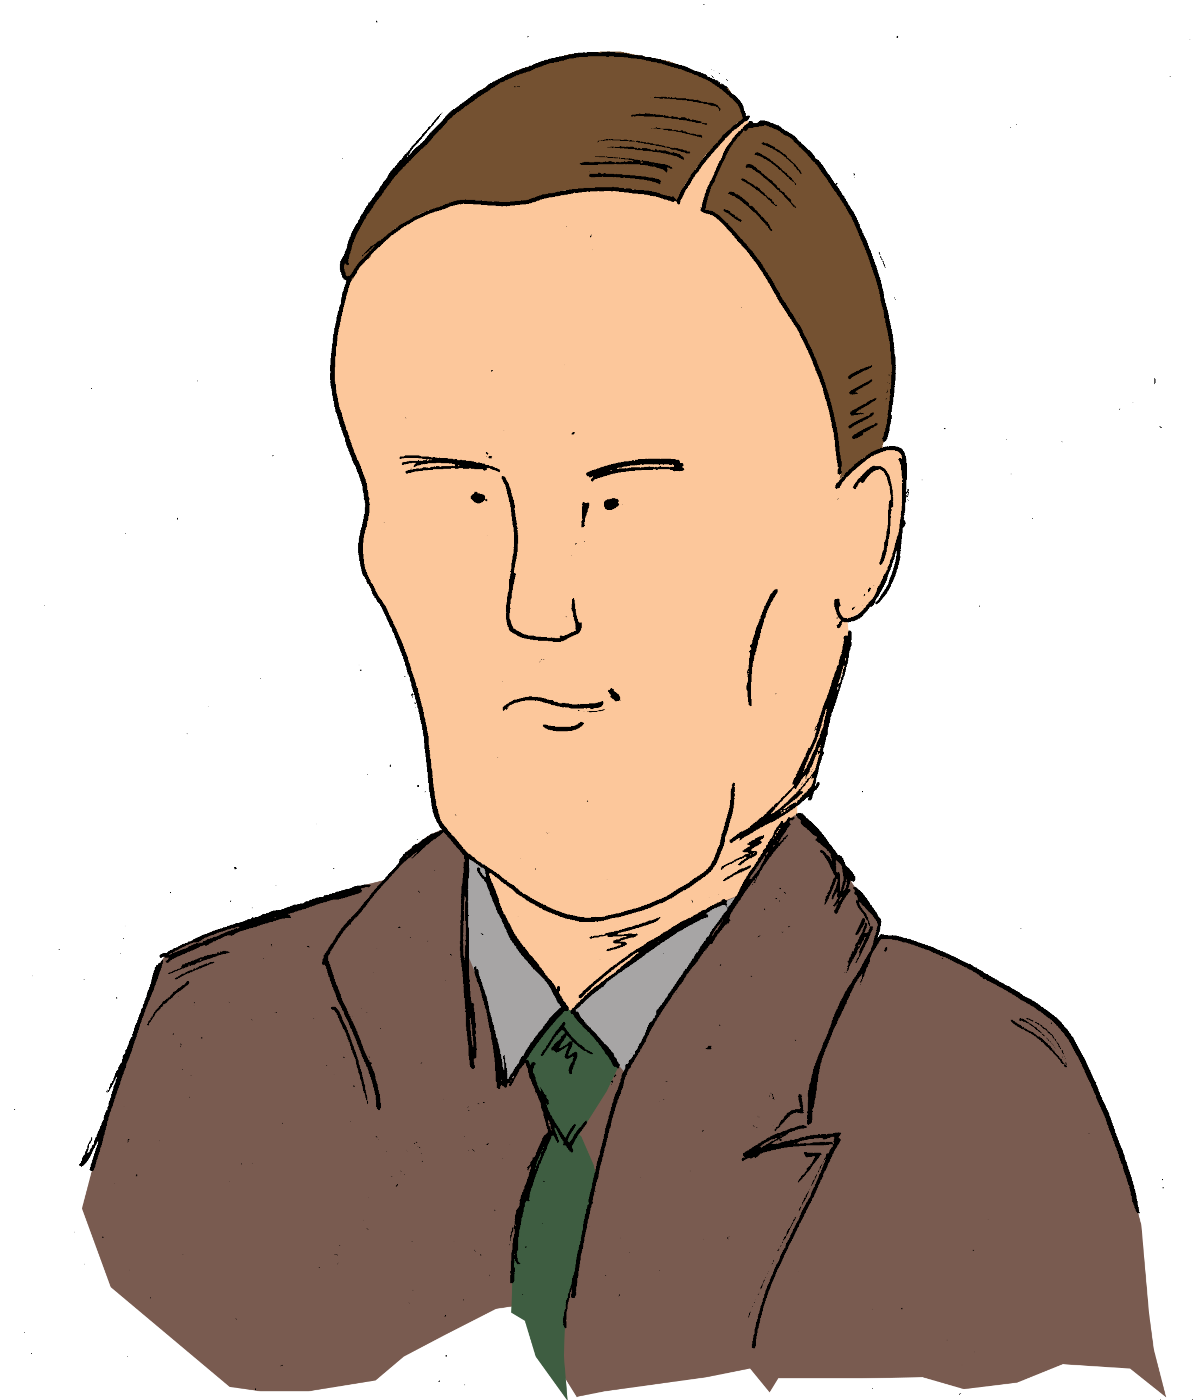
\includegraphics[width=8cm]{img/personaggi/alan_turing}};
			\node (example-textwidth-2) [notice={(-3,0.5)}, ultra thick, right, align=center, text width=12cm, color=black, fill=white, font=\fontsize{23pt}{24pt}\selectfont] at (12,-5) {Che cosa accadrà se una macchina prenderà il posto di A nel gioco? L'operatore darà una risposta errata altrettanto spesso di quando il gioco viene giocato tra un uomo e una donna?};
		\end{scope}
		%
		\begin{scope}[shift={(0,-88)}]
			\draw [fill=dida, ultra thick] (2,3.2) rectangle (12.5,1.7);
			\node (example-textwidth-2) [right, align=left, text width=25cm, color=black, font=\fontsize{23pt}{24pt}\selectfont] at (2.5,2.5) {O, piu' esplicitamente:};
			\node at (7,-4) {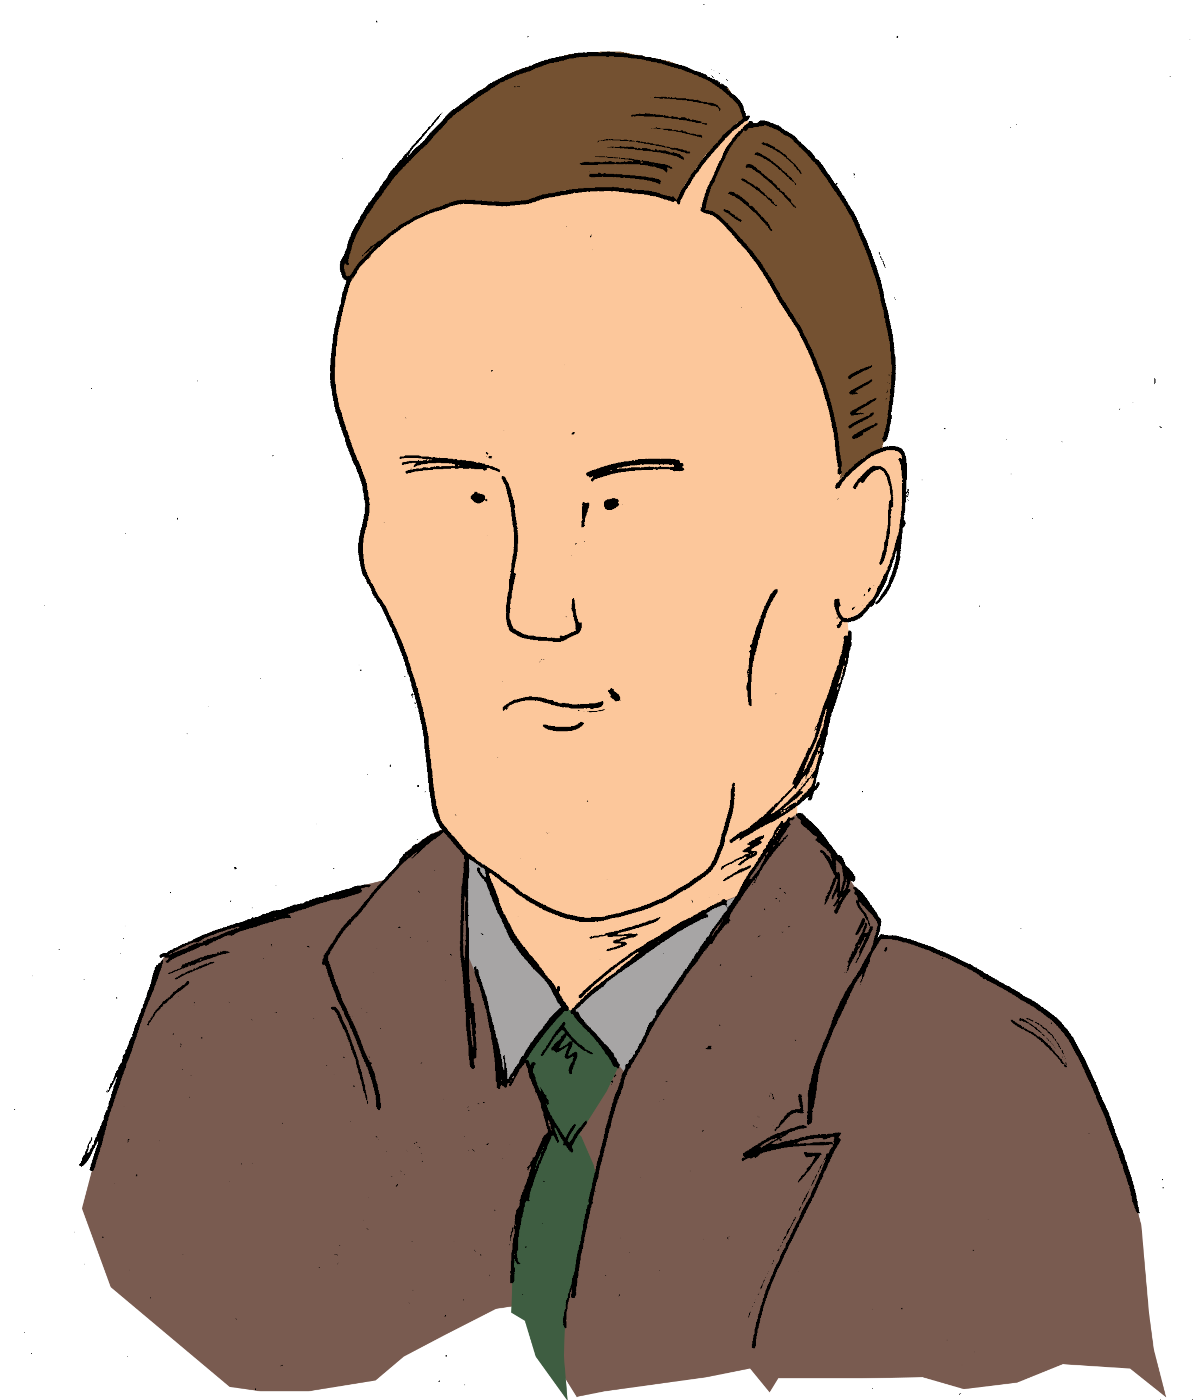
\includegraphics[width=8cm]{img/personaggi/alan_turing}};
			\node (example-textwidth-2) [notice={(-3,0.5)}, ultra thick, right, align=center, text width=12cm, color=black, fill=white, font=\fontsize{23pt}{24pt}\selectfont] at (12,-5) {Le macchine possono pensare?};
			\begin{scope}[shift=({21,-15})]
				\draw [fill=craterm] (3.9,0) -- (3.8,-2) -- (4.2,-2) -- (4.1,0) -- (3.9,0);
				\draw [fill=linem] (0,0) -- (0,4.5) -- (8,4.5) -- (8,0) -- (0,0);
				\draw [fill=craterm] (2.5,-2) -- (5.5,-2) -- (5.7,-2.1) -- (2.3,-2.1) -- (2.5,-2);
				\draw [fill=earth!50!white] (0.2,0.2) -- (0.2,4.3) -- (7.8,4.3) -- (7.8,0.2) -- (0.2,0.2);
				\draw [fill=white] (0.5,0.5) -- (0.5,4) -- (2.5,4) -- (2.5,0.5) -- (0.5,0.5);
				\foreach \i in {1,2,...,5}
				\draw (0.7,4-\i*0.2) -- (2.3-\i*0.1,4-\i*0.2);
			\end{scope}
			\node (example-textwidth-2) [notice={(3,0.5)}, ultra thick, right, align=center, text width=12cm, color=black, fill=white, font=\fontsize{23pt}{24pt}\selectfont] at (2,-16) {Se lo chiedete a me, si! Ma in fondo chi sono io se non una macchina?};
		\end{scope}
		%
		\begin{scope}[shift={(0,-107)}]
			\node at (27,0) () {
\includegraphics[width=3.7cm]{licenza}};
			\node at (27,0) () {
\includegraphics[width=3.7cm]{licenza}};
			\node at (18,-0.1) {\textcolor{black}{\fontsize{14}{15}\selectfont Testo e illustrazioni: @ulaulaman - Gianluigi Filippelli}};
		\end{scope}
	\end{tikzpicture}
\end{document}
